
\documentclass[a4paper,12pt]{article}

\usepackage{graphicx} % Required for inserting images
\usepackage{amsmath,amssymb,amsfonts}
\usepackage{subcaption}
% -----------------------
% Package Imports
% -----------------------

% Set page margins
\usepackage[a4paper, top=1in, bottom=0.8in, left=1.1in, right=0.8in]{geometry}

% Use Times New Roman font
\usepackage{times}

% Add page numbering
\pagestyle{plain}

% Enable graphics inclusion
\usepackage{graphicx}
\usepackage{float}
% Enable code listings
\usepackage{listings}
\usepackage{xcolor} % For customizing code colors
\setlength{\parindent}{0pt}
\usepackage{multirow}



\begin{document}
	\section{Experiment No. 3}
	
	\section{Experiment Title }
	Determination of synchronous reactance of a synchronous generator.
	
	\section{Objective}
	
	The objectives of this lab are as follows:
	\begin{itemize}
\item To determine the synchronous reactance of a synchronous generator through open circuit and short circuit tests.
\item To investigate the linearity of the open circuit voltage and short circuit current versus field current, and analyze the implications for estimating synchronous reactance
		
		
	\end{itemize}
	
	\section{Theory}
	
	Synchronous generators operate at synchronous speed to generate alternating current (AC) power at a desired frequency. An important parameter in analyzing their performance is the \textbf{synchronous reactance} ($X_s$), which represents the imaginary component of impedance that accounts for the voltage drop due to inductance in the generator.
	
	To determine $X_s$, two essential tests are performed:
	\begin{itemize}
		\item \textbf{Open Circuit Test (OCT)} – The generator is run at synchronous speed with no load connected. The terminal voltage ($E_{oc}$ or $V_{oc}$) is measured at different values of field current ($I_f$).
		\item \textbf{Short Circuit Test (SCT)} – The terminals are short-circuited and the short circuit current ($I_{sc}$) is measured for the same values of field current ($I_f$).
	\end{itemize}
	
	From the test data, the synchronous reactance can be determined using the ratio of open-circuit voltage to short-circuit current, assuming linear behavior and negligible armature resistance.
	
	\[
	X_s = \frac{V_{oc}}{I_{sc}}
	\]
	
	The phasor equation for a synchronous generator is:
	
	\[
	V_\phi = E_a - jX_s I_a - I_a R_a
	\]
	
	Where:
	\begin{itemize}
		\item $V_\phi$ = Phase voltage at the terminals
		\item $E_a$ = Induced EMF
		\item $I_a$ = Armature current
		\item $X_s$ = Synchronous reactance
		\item $R_a$ = Armature resistance
	\end{itemize}
	
	If the armature resistance $R_a$ is negligible, then:
	
	\[
	X_s = \frac{E_{oc}}{I_{sc}}
	\]
	
	This estimation aids in modeling and efficient operation of synchronous generators in power systems.
	
	
	
\begin{figure}[H]
	\centering

		\begin{subfigure}[t]{1\textwidth}
		\centering
		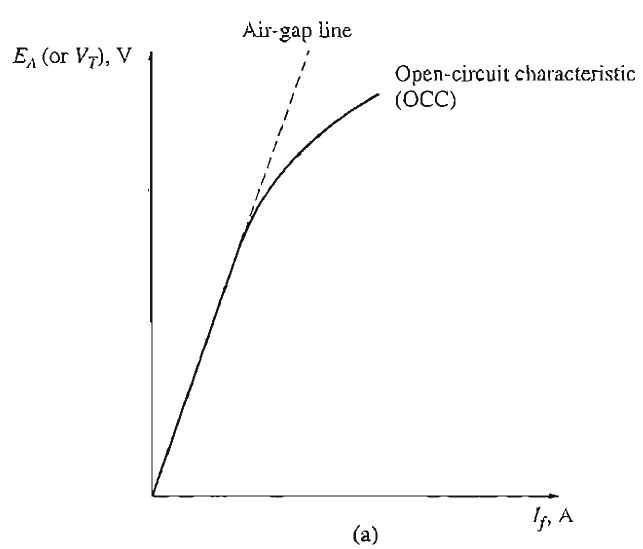
\includegraphics[width=0.5\linewidth]{Images/3}
		
		\vspace{2cm}
	\end{subfigure}
	
	\begin{subfigure}[t]{1\textwidth}
		\centering
		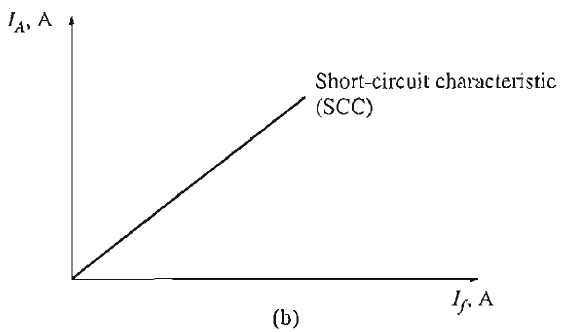
\includegraphics[width=0.5\linewidth]{Images/4}
		
	\end{subfigure}
		\caption{ Open Circuit Characteristic curve \& Short Circuit Characteristic Curve [Electric Machinery Fundamentals\_Chapman\_5ed]}
\end{figure}
\newpage
	\section{Circuit Diagram}
\begin{figure}[H]
	\centering
	\begin{subfigure}[t]{.9\textwidth}
		\centering
		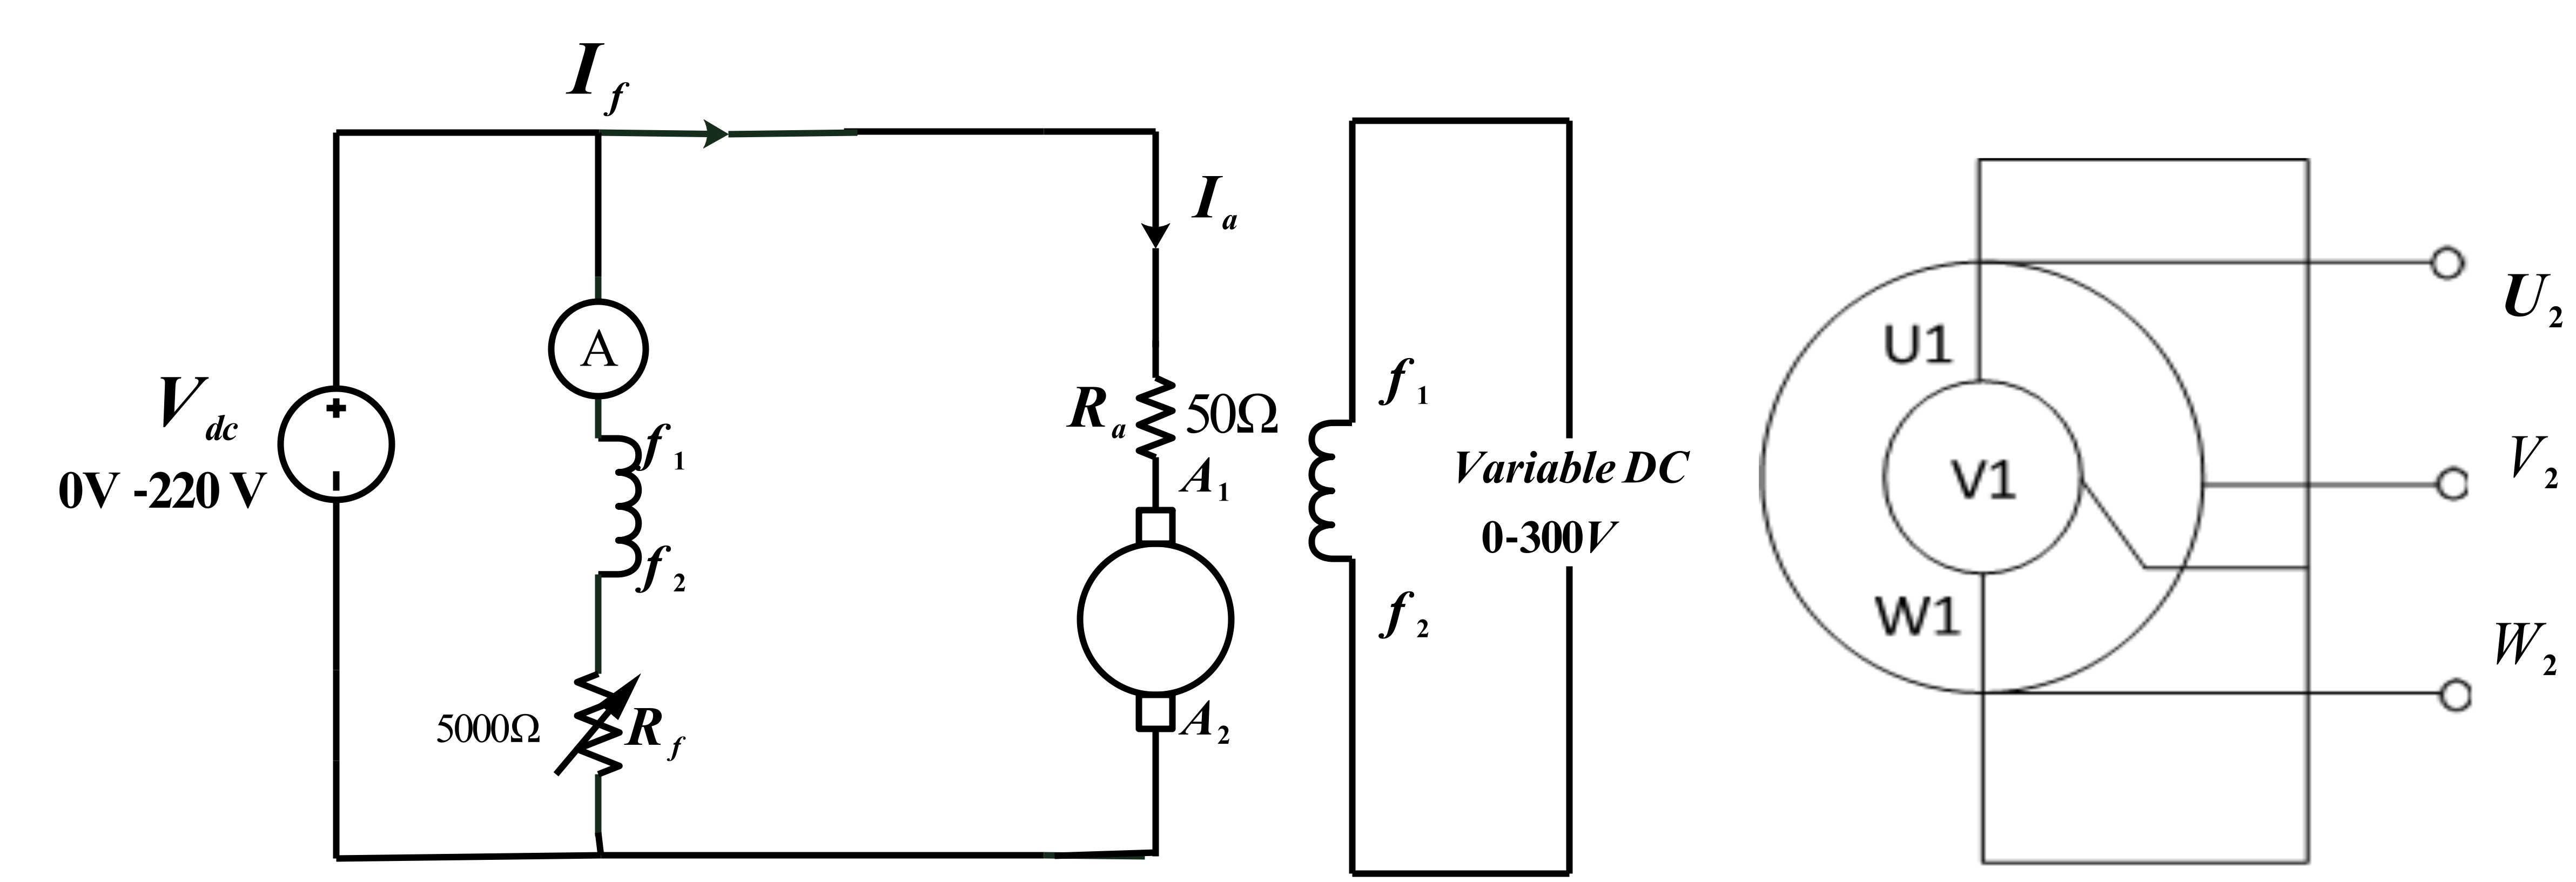
\includegraphics[width=1\textwidth]{Images/eee3108exp002}
		\caption{Circuit Diagram of Open Circuit Test.}
		
	\end{subfigure}
	\begin{subfigure}[t]{.9\textwidth}
		\centering
		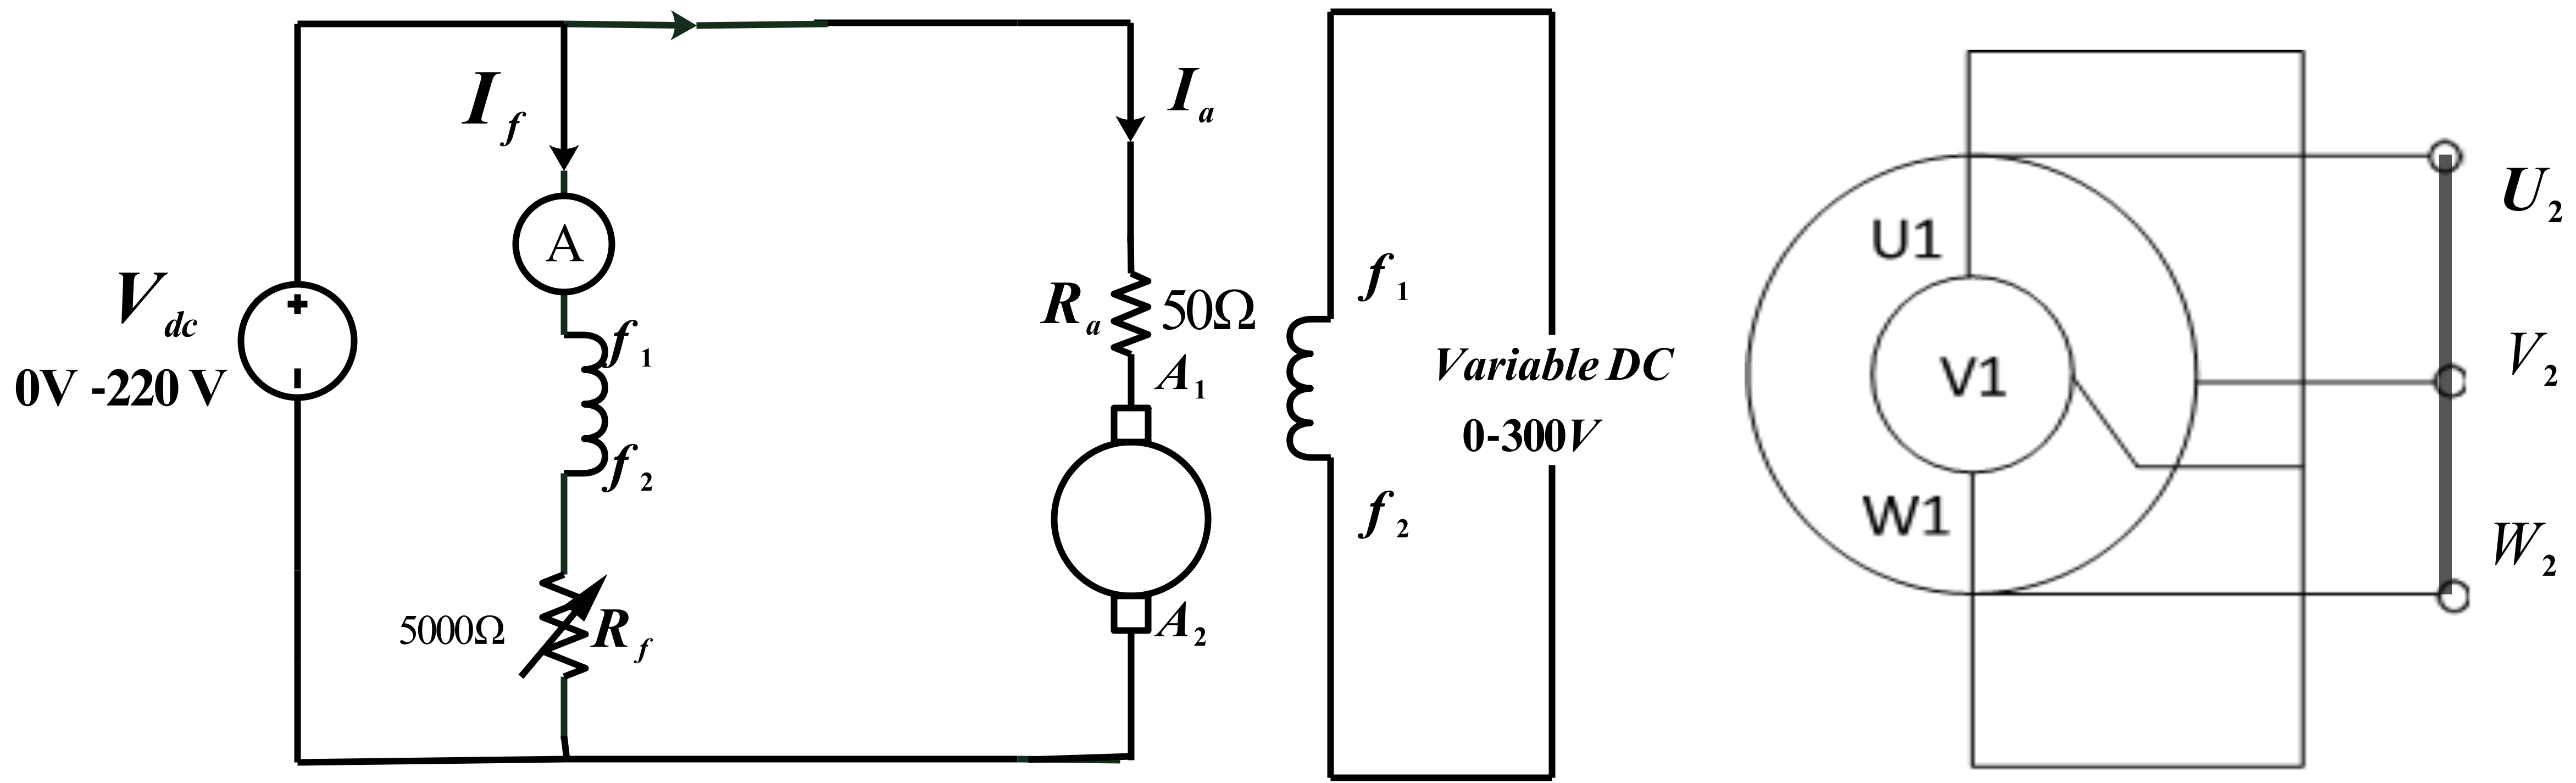
\includegraphics[width=1\textwidth]{Images/eee3108exp003}
		\caption{Circuit Diagram of Short Circuit Test.}
		
	\end{subfigure}
	
	
\end{figure}

\section{Required Apparatus}
\begin{enumerate}
	\item \textbf{DC Motor}
	\begin{enumerate}
		\item Power: 300W , Speed: 3000 rpm
		\item Voltage: 220V
		\item \textbf{Excitation (Series)}: D1-D2, Current: 1.9A, \textbf{Excitation (Separate)}: F1-F2, Current: 1.8A, Excitation Voltage: 220V, Excitation Current: 0.1A
		
	\end{enumerate}
	
	\item \textbf{Synchronous Generator}
	\begin{enumerate}
		\item Power: 350W ,Power Factor: $\cos\phi = 1$ ,Speed: 3000 rpm
		
		\item Voltage: 400V (star) / 230V (delta) ,Current: 0.7A (star) / 1.2A (delta) 
		\item Excitation Voltage: 220V ,Excitation Current: 0.45A
		
	\end{enumerate}
	
	\item \textbf{Resistors}
	\begin{enumerate}
		\item 50$\Omega$: Power = 500W, Current = 3.16A
		\item 200$\Omega$: Power = 500W, Current = 1.58A
		\item 5000$\Omega$: Power = 500W, Current = 0.31A
	\end{enumerate}
	
	\item \textbf{Tachometer}
	\begin{enumerate}
		\item For 0.6V/rev: 300V at 5000 RPM , For 2mV/rev: 10V at 5000 RPM
		\item Maximum Current: 0.07A
		\item Maximum Speed: 5000 RPM
	\end{enumerate}
	
	\item \textbf{AC Multimeter}
	\begin{enumerate}
		\item 500V AC RMS
		\item 5A
	\end{enumerate}
\end{enumerate}

	
	
	
	
	
	\section{Data Table}
% Please add the following required packages to your document preamble:
% \usepackage{multirow}
\begin{table}[H]
	\centering
	\caption{Readings of OCC \& SCC test}
	\begin{tabular}{|c|c|c|c|c|c|c|c|}
		\hline
		\begin{tabular}[c]{@{}c@{}}SI \\ No.\end{tabular} & $V_f$    & $I_{f}$    &$I_{sc}$   & $E_{oc}$   & $Z_s = \frac{E_{oc}}{I_{sc}} $ & $R_{eff}$                   & $X_s = \sqrt{Z^2 -R^2_{eff} }$  \\ \hline
				1                                                 & 37.2  & 0.068 & 0.133 & 85.2  & 640.600                     & \multirow{10}{*}{1.05} & 640.599 \\ \cline{1-6} \cline{8-8} 
				2                                                 & 48.10 & 0.089 & 0.168 & 112.2 & 667.857                     &                        & 667.856 \\ \cline{1-6} \cline{8-8} 
				3                                                 & 52.80 & 0.096 & 0.186 & 122.1 & 656.450                     &                        & 656.446 \\ \cline{1-6} \cline{8-8} 
				4                                                 & 60.58 & 0.109 & 0.212 & 140.4 & 662.264                     &                        & 662.263 \\ \cline{1-6} \cline{8-8} 
				5                                                 & 63.80 & 0.112 & 0.225 & 147.8 & 656.870                     &                        & 656.888 \\ \cline{1-6} \cline{8-8} 
				6                                                 & 66.10 & 0.116 & 0.236 & 154.4 & 654.237                     &                        & 654.236 \\ \cline{1-6} \cline{8-8} 
				7                                                 & 76.61 & 0.134 & 0.275 & 178.2 & 648.000                     &                        & 647.999 \\ \cline{1-6} \cline{8-8} 
				8                                                 & 80.70 & 0.143 & 0.286 & 190.5 & 666.084                     &                        & 666.083 \\ \cline{1-6} \cline{8-8} 
				9                                                 & 91.81 & 0.159 & 0.325 & 212.4 & 653.538                     &                        & 653.537 \\ \cline{1-6} \cline{8-8} 
				10                                                & 96.10 & 0.166 & 0.334 & 220.7 & 660.778                     &                        & 660.777 \\ \hline
			\end{tabular}
		\end{table}
		
		
\section{Graph}
\begin{figure}[H]
	\centering
	\begin{subfigure}[t]{1\textwidth}
		\centering
		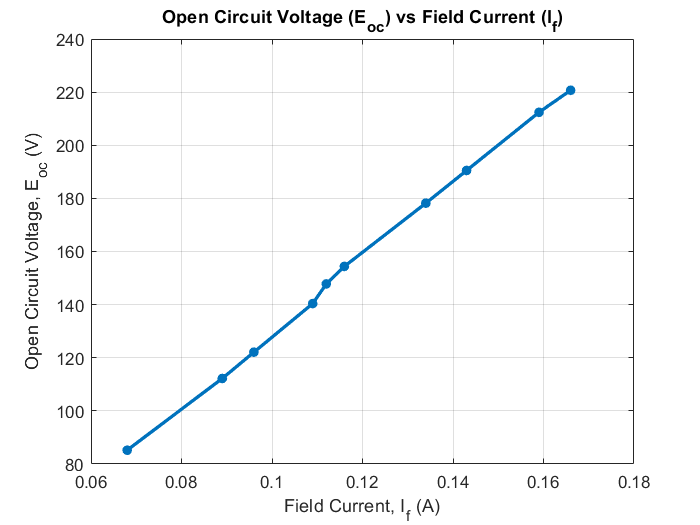
\includegraphics[width=.94\linewidth]{Images/1}
		\caption{$E_{oc}$ vs $I_f$ Graph }
		
	\end{subfigure}
	
	\begin{subfigure}[t]{1\textwidth}
		\centering
		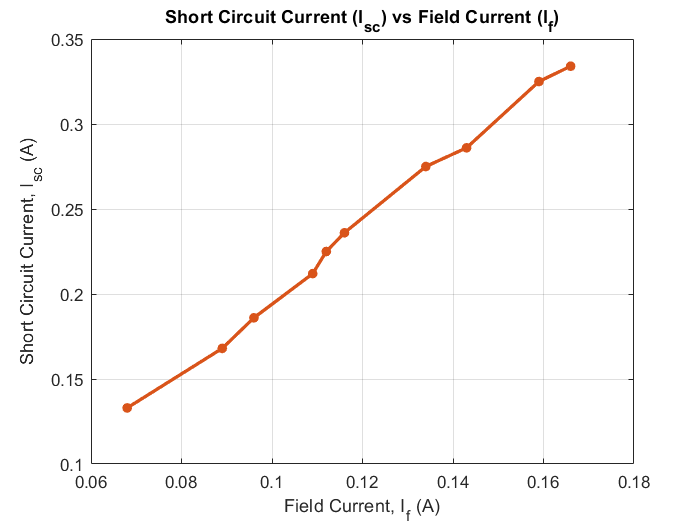
\includegraphics[width=.94\linewidth]{Images/2}
		\caption{ $I_{sc}$ vs $I_f$ Graph}
	\end{subfigure}
	
	
\end{figure}

\section{Discussion}
		
		
		The synchronous reactance of the generator was found by performing Open Circuit and Short Circuit tests with different field currents. In the Open Circuit Test, the terminal voltage was seen to increase almost linearly with the field current in the unsaturated region, following the Open Circuit Characteristic (OCC):
		
		\[
		E_{oc} \propto I_f
		\]
		
		In the Short Circuit Test, the short-circuit current also rose linearly with the field current, as magnetic saturation was minimal.
		
		The synchronous reactance ($X_s$) was calculated by taking the ratio of the open-circuit voltage to the short-circuit current:
		
		\[
		X_s = \frac{V_{oc}}{I_{sc}}
		\]
		
		The results matched the expected result, confirming the method and showing the dependence of $X_s$ on excitation and magnetic properties. Overall, the experiment was completed successfully, and synchronous reactance was determined.
		
\end{document}